\chapter{Lecture 8: New Revolutions in Particle Physics and the Higgs Mechanism}

These notes follow Leonard Susskind's eighth lecture in the supplementary Particle Physics 2 Standard Model course. The problem is stated carefully at the outset. We are not going to give a mass to the real photon, because real electromagnetism is not spontaneously broken. Instead we use the photon as the simplest toy model for the general question: how can a gauge boson acquire a mass when the symmetry associated with it is spontaneously broken? The lecture unfolds in a definite order. First we pin down what ``mass'' means for a field mode. Then we build the broken scalar theory. Then we review gauge invariance. Only after that do we put the two pieces together. These companion notes preserve that progression, with curation by LazyingArt LLC.

\section{Why Use the Photon as the Toy Model?}

The lecture begins by correcting a slogan. One often hears that the Higgs mechanism gives mass to the photon, but that is not the physical content of the Standard Model. The real photon remains massless. What we study instead is a deliberately simplified abelian model in which the symmetry associated with electric charge, namely a \(U(1)\) phase rotation, is imagined to break spontaneously. In that world the gauge boson would behave as a massive particle.

That is why the photon is a useful rehearsal. The actual electroweak story involves the \(W\) and \(Z\) bosons and a more intricate nonabelian symmetry, but the abelian case lets us see the core mechanism before the algebra becomes crowded.

Susskind immediately anchors the discussion in physics we already know. There is a place in nature where the photon behaves as if it had a mass: inside a superconductor. When the photon leaves the superconductor it is again an ordinary massless photon, but inside the material the propagation law is different. This is the first concrete example of the Higgs phenomenon.

He also inserts a brief motivational aside that should not be lost. Not every particle need owe its mass to spontaneous symmetry breaking. Some particles may have large ``natural'' masses for other reasons, and if so they are likely to live at scales far above the particles that dominate ordinary laboratory physics. The particles we do see---the light ones, and in particular the gauge bosons of the Standard Model---are exactly the ones for which symmetry can forbid a mass until the symmetry is broken. That is why this toy problem matters.

\subsection{Question \& Answer}

\paragraph{Question.} Why is a photon in a prism still massless, while a photon in a superconductor behaves as if it has a mass?

\paragraph{Answer.} Because a reduced propagation speed is not the same thing as a nonzero rest energy. In a prism the slope of the dispersion curve changes, but the curve still passes through the origin. At zero momentum, or equivalently infinite wavelength, the frequency is still zero. In a superconductor the relevant mode no longer has zero frequency at zero momentum. That is the operative sign of a mass. Throughout the lecture, this is the criterion that matters.

\section{Mass, Dispersion, and Flat Directions}

Before we touch the Higgs field itself, the lecture insists on a kinematic point. What does it mean for a wave or field excitation to be massless? What does it mean for it to be massive? The answer is given in terms of the dispersion relation, the relation between frequency and wave number.

We start from
\begin{equation}
E=\hbar\omega,
\qquad
p=\hbar k.
\end{equation}
So the graph of \(E\) versus \(p\) and the graph of \(\omega\) versus \(k\) differ only by factors of \(\hbar\). For a massless wave in empty space,
\begin{equation}
\omega = ck.
\end{equation}
This is linear. In particular, \(\omega=0\) when \(k=0\). The slope of the curve,
\begin{equation}
v=\frac{d\omega}{dk},
\end{equation}
is the propagation velocity. When the slope is constant, all wavelengths move with the same speed and there is no dispersion.

For a massive particle the energy-momentum relation is different:
\begin{equation}
E^2 = c^2p^2 + m^2c^4.
\end{equation}
Setting \(c=1\) gives
\begin{equation}
E^2 = p^2 + m^2.
\end{equation}
In the corresponding natural units for waves, the same structure is
\begin{equation}
\omega^2 = k^2 + m^2.
\end{equation}
Now the crucial point is obvious: when \(k=0\), the frequency is not zero. It is \(m\). That is what the mass is.

\begin{figure}[t]
\centering
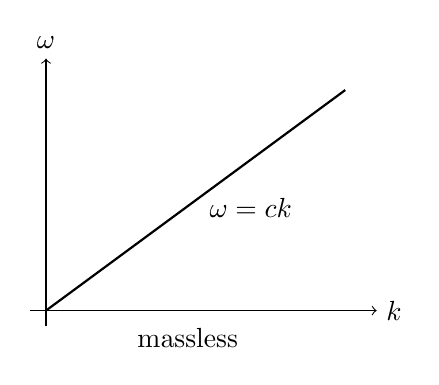
\begin{tikzpicture}[scale=1.0]
\draw[->] (-0.2,0) -- (4.2,0) node[right] {$k$};
\draw[->] (0,-0.2) -- (0,3.2) node[above] {$\omega$};
\draw[thick] (0,0) -- (3.8,2.8);
\node at (2.6,1.3) {$\omega = ck$};
\node at (1.8,-0.35) {massless};
\end{tikzpicture}
\hspace{1.2cm}
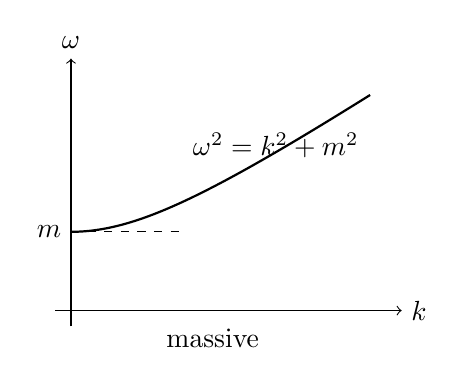
\begin{tikzpicture}[scale=1.0]
\draw[->] (-0.2,0) -- (4.2,0) node[right] {$k$};
\draw[->] (0,-0.2) -- (0,3.2) node[above] {$\omega$};
\draw[thick,domain=0:3.8,samples=100,smooth] plot (\x,{sqrt(1.0+0.45*\x*\x)});
\draw[dashed] (0,1.0) -- (1.4,1.0);
\node[left] at (0,1.0) {$m$};
\node at (2.6,2.1) {$\omega^2 = k^2 + m^2$};
\node at (1.8,-0.35) {massive};
\end{tikzpicture}
\caption{Transcript-guided redraw of the two dispersion relations that organize the opening discussion. The prism changes the slope of the massless line; it does not create a nonzero intercept at \(k=0\).}
\end{figure}

This is already field theory in embryo. The limit \(k=0\) means infinite wavelength. Infinite wavelength means that the whole field is displaced homogeneously, every point in space being shifted in the same way. If we shift the field everywhere and let it go, then a massive field oscillates with nonzero frequency, while a massless field does not.

That brings us to the next bridge in the lecture: the curvature of the potential. If the potential curves upward at equilibrium, a homogeneous displacement is pulled back and oscillates. If the potential is flat in a certain direction, a homogeneous displacement in that direction simply sits there. Thus mass becomes a geometric statement:

\begin{itemize}
\item curvature of the potential at equilibrium gives a massive mode;
\item a flat direction of the potential gives a massless mode.
\end{itemize}

This is the clue that prepares the broken-symmetry potential. Once the minimum is not a point but a whole rim, motion around the rim is massless while motion normal to it is massive.

\section{Complex Scalar Field and the Broken \(U(1)\) Potential}

The lecture now introduces the field that will carry the broken symmetry. We take a complex scalar field \(\phi\). In Cartesian variables,
\begin{equation}
\phi = \phi_R + i\phi_I,
\qquad
\phi^* = \phi_R - i\phi_I.
\end{equation}
In polar variables,
\begin{equation}
\phi = \rho e^{i\alpha},
\qquad
\phi^* = \rho e^{-i\alpha}.
\end{equation}
These are two descriptions of the same field. The variables \(\rho\) and \(\alpha\) are coordinates in field space, not in ordinary space. At each point of space-time, the field takes a value, and that value can be plotted as a point in the complex plane.

\begin{equation}
\phi^*\phi=\rho^2=\phi_R^2+\phi_I^2.
\end{equation}

\begin{figure}[t]
\centering

\includegraphics[width=0.62\textwidth]{lecture_08_figure_02.png}
\caption{The lecture's internal-space sketch of the complex field. The visible labels \(\phi_R\), \(\phi_I\), \(\rho\), and \(\alpha\) are the essential pieces of notation.}
\end{figure}

\begin{figure}[t]
\centering
\begin{tikzpicture}[scale=1.3]
\draw[->] (-0.3,0) -- (3.3,0) node[right] {$\phi_R$};
\draw[->] (0,-0.3) -- (0,2.8) node[above] {$\phi_I$};
\draw[thick] (0,0) -- (2.5,1.7);
\draw (0.78,0) arc (0:34:0.78);
\node at (1.65,1.15) {$\rho$};
\node at (1.02,0.33) {$\alpha$};
\fill (2.5,1.7) circle (1.4pt);
\end{tikzpicture}
\caption{A clean redraw of the same field-space geometry.}
\end{figure}

The kinetic term may be written in either language. In Cartesian form,
\begin{equation}
\partial_\mu\phi^*\,\partial^\mu\phi
=
\partial_\mu\phi_R\,\partial^\mu\phi_R
+
\partial_\mu\phi_I\,\partial^\mu\phi_I.
\end{equation}
So a complex scalar field is, in one sense, simply two real scalar fields written compactly. In polar variables the same term becomes
\begin{equation}
\partial_\mu\phi^*\,\partial^\mu\phi
=
\partial_\mu\rho\,\partial^\mu\rho
+
\rho^2\,\partial_\mu\alpha\,\partial^\mu\alpha.
\end{equation}
This is the version the lecture wants, because it separates radial motion from angular motion.

A \(U(1)\)-symmetric potential depends only on \(\rho\), or equivalently only on \(\phi^*\phi\):
\begin{equation}
V=V(\rho)=V(\phi^*\phi).
\end{equation}
It does not depend on the angle \(\alpha\). If the potential were simply quadratic,
\begin{equation}
V(\rho)\propto \rho^2 = \phi_R^2+\phi_I^2,
\end{equation}
then both directions would be massive. That is the unbroken case. But the lecture wants the other possibility: a potential whose minimum lies at nonzero radius \(\rho=f\). Then the angular direction is flat and the radial direction is curved. The natural coordinates are now \(\rho\) and \(\alpha\), not \(\phi_R\) and \(\phi_I\).

\begin{figure}[t]
\centering

\includegraphics[width=0.8\textwidth]{lecture_08_figure_03.png}
\caption{Board layout for the radially symmetric potential discussion. The mathematical point is carried by the potential sketches and the label \(V(\phi)\), not by the numerical examples at the far right.}
\end{figure}

\begin{figure}[t]
\centering
\begin{tikzpicture}[scale=1.0]
\draw[->] (-0.2,0) -- (4.5,0) node[right] {$\rho$};
\draw[->] (0,-0.2) -- (0,3.2) node[above] {$V(\rho)$};
\draw[thick,domain=0:4.2,samples=120,smooth]
plot (\x,{0.18*(\x-2.2)^4 - 0.95*(\x-2.2)^2 + 1.7});
\draw[dashed] (2.2,0) -- (2.2,0.35);
\node[below] at (2.2,0) {$f$};
\end{tikzpicture}
\hspace{1.2cm}
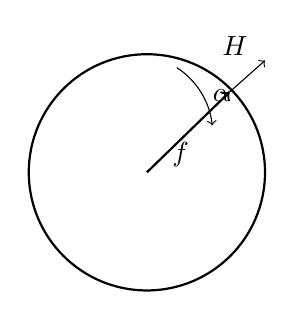
\begin{tikzpicture}[scale=1.0]
\draw[thick] (0,0) circle (1.5);
\draw[thick,->] (0,0) -- (1.05,1.02);
\draw[->] (0.38,1.33) arc (57:6:1.0);
\draw[->] (1.05,1.02) -- (1.5,1.42);
\node at (0.43,0.22) {$f$};
\node at (0.95,0.98) {$\alpha$};
\node at (1.12,1.6) {$H$};
\end{tikzpicture}
\caption{A clean reconstruction of the broken potential: a radial slice with minimum at \(\rho=f\), and a schematic rim showing the flat angular direction and the radial Higgs fluctuation.}
\end{figure}

\subsection{Question \& Answer}

\paragraph{Question.} What is radially symmetric here: the field itself or the potential energy?

\paragraph{Answer.} The potential energy. The field at a given point of space-time is just a value, that is, a point in the complex plane. There is nothing radially symmetric about that single value. What is radially symmetric is the rule that assigns potential energy to field values. That rule depends only on \(\phi^*\phi=\rho^2\), so two points on the same circle have the same potential energy.

\section{Low-Energy Modes: Higgs and Goldstone}

Once the minimum sits at nonzero radius, the lecture identifies the two kinds of motion. Radial motion changes \(\rho\) and climbs the potential. Angular motion changes \(\alpha\) and moves around the flat rim. It is therefore natural to write
\begin{equation}
\rho = f + H,
\end{equation}
where \(H\) is the fluctuation of the radial coordinate away from the minimum. This is the Higgs mode.

The lecture makes the physical hierarchy explicit. The radial direction is steep. It costs a good deal of energy to excite \(H\). The angular direction is flat. It costs no potential energy at all to move around the rim. So in this broken scalar theory there are two types of quanta:

\begin{itemize}
\item the radial Higgs mode, which is massive;
\item the angular Goldstone mode, which is massless.
\end{itemize}

At low energy we may neglect the heavy radial excitation and freeze the field near the minimum:
\begin{equation}
\rho \approx f,
\qquad
\partial_\mu\rho \approx 0,
\qquad
V(\rho)\approx V(f).
\end{equation}
The potential term is then just a constant, and the radial kinetic term drops out. What remains is
\begin{equation}
\mathcal L_{\mathrm{low}}
\approx
f^2\,\partial_\mu\alpha\,\partial^\mu\alpha.
\end{equation}
There is no mass term for \(\alpha\). The energy comes only from derivatives. If \(\alpha\) is displaced homogeneously everywhere, nothing happens. This is exactly the hallmark of a massless field.

To bring the normalization into a more familiar form, the lecture rescales the field:
\begin{equation}
\beta = f\alpha.
\end{equation}
Then
\begin{equation}
\mathcal L_{\mathrm{low}}
\approx
\partial_\mu\beta\,\partial^\mu\beta.
\end{equation}
So the Goldstone boson is just a massless scalar field written in the variables natural to the broken vacuum.

This is the point at which Susskind says, in effect, that we have only half the story. Spontaneous symmetry breaking plus a continuous symmetry gives a Goldstone boson. But the Higgs mechanism is not merely the Goldstone theorem. We still need the other half: gauge invariance.

\section{From Global \(U(1)\) to Local Gauge Invariance}

After the break the lecture deliberately slows down. There is real confusion in the room about what a complex field is, so Susskind reviews it: the complex plane is not physical space; it is an auxiliary plane in which the field value is plotted. Once that is clear, one can ask what it means to rotate the field.

A global \(U(1)\) transformation rotates the field by the same phase everywhere:
\begin{equation}
\phi(x)\to e^{i\theta}\phi(x),
\qquad
\theta=\text{constant}.
\end{equation}
This shifts \(\alpha\) by a constant and leaves \(\rho\) unchanged. Since the potential depends only on \(\rho\), and derivatives annihilate constants, the Lagrangian is unchanged.

What fails is the local version,
\begin{equation}
\phi'(x)=e^{i\theta(x)}\phi(x).
\end{equation}
Now the derivative acts on \(\theta(x)\) as well as on \(\phi\):
\begin{align}
\partial_\mu\phi'
&=
\partial_\mu\!\left(e^{i\theta(x)}\phi\right) \\
&=
e^{i\theta(x)}
\left(
\partial_\mu\phi+i(\partial_\mu\theta)\phi
\right).
\end{align}
The extra term proportional to \(\partial_\mu\theta\) is the obstruction. It is exactly the term Susskind calls the nuisance.

\begin{figure}[t]
\centering

\includegraphics[width=0.78\textwidth]{lecture_08_figure_04.png}
\caption{The blackboard moment in which the local phase rotation is tried and found to be ``not sym.'' The derivation on the board is schematic, and the cleaned indexed formulas are given in the text.}
\end{figure}

At the board the conclusion is stated schematically as
\begin{equation}
\partial\phi^*\,\partial\phi
\neq
\partial\phi^{*\prime}\,\partial\phi'.
\end{equation}
That is the right lesson. The board notation suppresses Lorentz indices, so in the chapter we restore them and choose a consistent convention. The lecture itself wobbles on the signs, and Susskind says so, so from here onward we fix
\begin{equation}
D_\mu\phi=(\partial_\mu+iA_\mu)\phi,
\qquad
D_\mu\phi^*=(\partial_\mu-iA_\mu)\phi^*,
\end{equation}
together with
\begin{equation}
A'_\mu=A_\mu-\partial_\mu\theta.
\end{equation}
Then the transformed covariant derivative is
\begin{align}
D'_\mu\phi'
&=
(\partial_\mu+iA'_\mu)e^{i\theta}\phi \\
&=
e^{i\theta}\left(\partial_\mu+iA_\mu\right)\phi \\
&=
e^{i\theta}D_\mu\phi.
\end{align}
The derivative of \(\theta\) has disappeared. That is the whole point of the compensating field \(A_\mu\).

The gauge field has its own gauge-invariant curvature,
\begin{equation}
F_{\mu\nu}=\partial_\mu A_\nu-\partial_\nu A_\mu.
\end{equation}
Under the same transformation,
\begin{align}
F'_{\mu\nu}
&=
\partial_\mu A'_\nu-\partial_\nu A'_\mu \\
&=
F_{\mu\nu}
-\partial_\mu\partial_\nu\theta
+\partial_\nu\partial_\mu\theta \\
&=
F_{\mu\nu},
\end{align}
because mixed partial derivatives commute. This is the board argument behind the statement \(F'=F\).

The lecture summarizes the theory schematically as
\begin{equation}
\mathcal L_{\mathrm{toy}}
=
D\phi^*\,D\phi - V(\phi^*\phi) + F^2.
\end{equation}
As written on the board this is shorthand, not an attempt at textbook normalization. In explicit notation we may read the same structure as
\begin{equation}
\mathcal L_{\mathrm{toy}}
=
D_\mu\phi^*\,D^\mu\phi
-
V(\phi^*\phi)
+
F_{\mu\nu}F^{\mu\nu},
\end{equation}
with the understanding that the Maxwell term was kept schematic in the lecture.

\begin{figure}[t]
\centering

\includegraphics[width=0.78\textwidth]{lecture_08_figure_05.png}
\caption{A secondary board summary showing the schematic gauge-invariant scalar-gauge Lagrangian together with the remembered expansion \(\rho=f+H\). This frame is useful as a summary surface, not as direct evidence for the forbidden \(A_\mu A^\mu\) term.}
\end{figure}

\subsection{Question \& Answer}

\paragraph{Question.} Why is the local phase rotation not already a symmetry of the scalar kinetic term?

\paragraph{Answer.} Because \(\partial_\mu\) differentiates every \(x\)-dependence in sight. If \(\theta\) is constant, the derivative never sees it and the phase simply factors out. If \(\theta=\theta(x)\), the derivative produces the extra term \(i(\partial_\mu\theta)\phi\). That term spoils the transformation of the ordinary kinetic term. The gauge field and the covariant derivative are introduced precisely to cancel it.

\section{The Higgs Mechanism in the Toy Gauge Theory}

Now we put the two halves together. Up to this point there seem to be two massless things in the theory. The broken scalar sector contains the Goldstone boson. The gauge sector contains the photon, which is massless because its energy depends only on derivatives of \(A_\mu\). In Susskind's language, there are two massless particles floating around, and now we are to watch what happens.

First, why can we not simply give the photon a mass by hand? Because the obvious mass term would be
\begin{equation}
A_\mu A^\mu.
\end{equation}
Under a gauge transformation,
\begin{equation}
A_\mu A^\mu
\;\longrightarrow\;
(A_\mu-\partial_\mu\theta)(A^\mu-\partial^\mu\theta),
\end{equation}
and that is not the same expression. So gauge invariance forbids a direct mass term.

But this does not settle the matter. The lecture now asks us to look more closely at the covariant-derivative term in the broken phase. At low energy we freeze the radial mode and write
\begin{equation}
\phi(x)\approx f e^{i\alpha(x)}.
\end{equation}
Then
\begin{align}
D_\mu\phi
&\approx
(\partial_\mu+iA_\mu)\bigl(f e^{i\alpha}\bigr) \\
&=
i f e^{i\alpha}\bigl(\partial_\mu\alpha + A_\mu\bigr).
\end{align}
Hence
\begin{equation}
|D_\mu\phi|^2
\approx
f^2\bigl(\partial_\mu\alpha + A_\mu\bigr)
\bigl(\partial^\mu\alpha + A^\mu\bigr).
\end{equation}
This is the decisive combination. The lecture reaches it somewhat wearily and with sign hesitation on the board, but the structure is clear.

\begin{figure}[t]
\centering

\includegraphics[width=0.62\textwidth]{lecture_08_figure_06.png}
\caption{In-progress board substitution of the frozen-\(\rho\) field into the covariant derivative. The right-hand side is cut off in the frame, so the cleaned algebra is reconstructed in the text rather than read literally from the screenshot.}
\end{figure}

Now choose the gauge function to be
\begin{equation}
\theta(x)=-\alpha(x).
\end{equation}
With our fixed convention,
\begin{equation}
\phi'(x)=e^{i\theta(x)}\phi(x)=f,
\qquad
A'_\mu=A_\mu+\partial_\mu\alpha.
\end{equation}
So the angular field disappears from the scalar, and the covariant-derivative term reduces to
\begin{equation}
|D_\mu\phi|^2 \to f^2 A'_\mu A^{\mu\prime}.
\end{equation}
That is precisely a mass term for the gauge field. It has emerged from a gauge-invariant expression after the vacuum settled at nonzero \(\rho\). We did not add the forbidden term \(A_\mu A^\mu\) by hand. We generated it dynamically through the covariant derivative.

This is the abelian Higgs mechanism. The lecture at one point says this loosely as though the Goldstone boson were eaten and the Higgs boson thereby gained its mass. The calculation makes the physics sharper: the new mass term is for the gauge boson, while the radial Higgs mode is already the massive direction of oscillation about the broken vacuum.

The condensed-matter analogy now falls into place. In a superconductor there is a charged bosonic condensate, built physically from Cooper pairs. The field describing that condensate plays the role of \(\phi\). Once it condenses, the electromagnetic field inside the superconductor behaves as in this toy model: the photon acquires an effective mass.

\subsection{Question \& Answer}

\paragraph{Question.} Where did the Goldstone boson go, and how can no degree of freedom be lost?

\paragraph{Answer.} The Goldstone boson was the phase field \(\alpha(x)\). But in the gauged theory a space-time dependent change of phase is exactly what a gauge transformation does. So the would-be Goldstone mode is not an independent physical excitation once the symmetry is gauged. It is absorbed into the gauge field and reappears as the longitudinal polarization of the now-massive vector boson.

This is the degree-of-freedom counting emphasized at the end of the lecture:
\begin{equation}
2\ \text{(massless photon polarizations)}
+
2\ \text{(real scalar components)}
\;\longrightarrow\;
3\ \text{(massive vector polarizations)}
+
1\ \text{(Higgs scalar)}.
\end{equation}
A massless photon has only two transverse polarizations because it can never be brought to rest. A massive vector boson can be brought to rest, and then there is no reason to exclude a longitudinal polarization. That missing third polarization is exactly what the Goldstone mode becomes.

\section{Summary}

The lecture unfolds as a single argument rather than as a list of facts. We begin by learning what mass means: it is the nonzero frequency of the homogeneous \(k=0\) mode. That kinematic statement becomes a field-theoretic one when we connect mass to curvature of the potential. A broken \(U(1)\)-symmetric scalar potential therefore gives a heavy radial Higgs mode and a massless angular Goldstone mode.

That is only half the story. The other half is gauge invariance. A local phase rotation is not a symmetry of the ordinary derivative term, so we introduce the vector potential, the covariant derivative, and the field strength. Once the scalar field sits at nonzero magnitude, the covariant derivative produces the combination \(\partial_\mu\alpha + A_\mu\). A gauge choice removes \(\alpha\), and what remains is an effective mass term for the gauge field. The Goldstone boson has not vanished; it has become the longitudinal polarization of the massive vector boson. That is the simple abelian version of the Higgs mechanism, and it is the clean toy model for the gauge-boson masses of the Standard Model.